\documentclass[a4paper,11pt]{paper}

\usepackage[pdftex]{graphicx}

\title{ColouredTree: a BEAST 2 framework for describing
phylogenies within structured populations}

\author{Tim Vaughan}

\newcommand{\class}[1]{\textsf{#1}}
\newcommand{\project}[1]{\textsf{#1}}

\begin{document}

\maketitle

\section{Introduction}

BEAST 2 (hereafter simply referred to as BEAST) currently provides no
native way of handling true coloured trees---i.e., phylogenetic trees
corresponding to lineages evolving within some kind of structured
population. While it is true that BEAST has a useful facility for
recording arbitrary metadata in the form of ``traits'' on tree nodes,
information cannot be modified by BEAST Operators.  Without this
capability, geographic model parameters such as migration rates are
beyond the scope of the inference apparatus.

This document describes some first steps towards addressing these
shortcommings.

\section{State of the project}
Before going into the details of the plugin itself, let's consider the
current state of the development. So far, we have in place
\begin{itemize}
	\item a plugin for representing coloured trees,
	\item a plugin for initialising coloured trees from the structured
		coalescent, and
	\item a means of visualising coloured trees using Alexei's
		\project{beast-graphics} project.
\end{itemize}
These are the items which are described in the present document.

On the to-do list are the following (more challenging) items:
\begin{itemize}
	\item proposal operators for modifying colour assignments,
	\item calculation nodes for determining likelihoods of particular
		colour assignments.
\end{itemize}
Note that specific likelihoods and proposal operators depend on the
underlying structural model the colours represent, so we firstly need
to implement a general framework for such operators, then implement
some specific common cases (such as those relating to models of
migration between demes).

\section{Implementation of Coloured Trees (ColouredTree plugin)}

The first and most important point about the way in which coloured
trees are implemented is that the main class, \class{ColouredTree},
extends \class{Plugin}---it does not extend \class{Tree}.  As such,
\class{ColouredTree}s are not \class{StateNodes}, and cannot be used
directly in an MCMC calculation.  Instead, \class{ColouredTree} takes
a \class{Tree} as an input, along with the following three parameters:
\begin{description}
	\item[\class{changeCounts}]: an \class{IntegerParameter} array which
		is used to record the number of 
\end{description}

\subsection{ColouredTree inputs}

\subsection{ColouredTree methods}

\begin{figure}
	\centering
	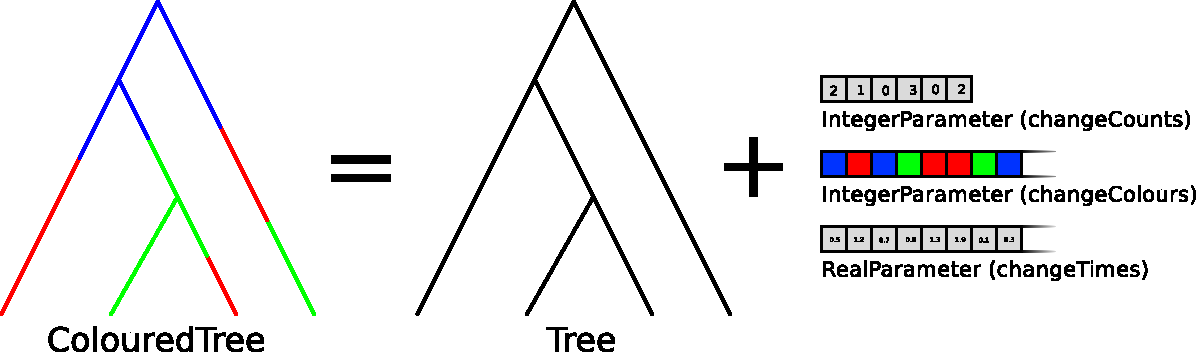
\includegraphics[width=\textwidth]{treeComposition.pdf}
	\caption{Composition of the \class{ColouredTree} plugin.}
\end{figure}

\section{Generating Coloured Trees (StructuredCoalescentColouredTree plugin)}

\subsection{StructuredCoalescentColouredTree inputs}
\subsection{StructuredCoalescentColouredTree methods}

\begin{figure}
	\centering
	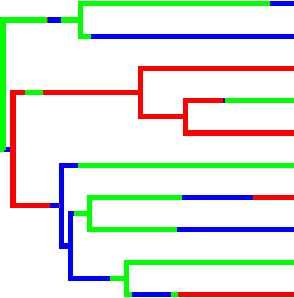
\includegraphics[width=0.5\textwidth]{structuredCoalescentFig.pdf}
	\caption{Coloured tree generated using
		\class{StructuredCoalescentColouredTree} and visualised using
	\project{beast-graphics}.}
\end{figure}

\section{Interfacing with {\textsf beast-graphics} (FlatColouredTree plugin)}

\subsection{FlatColouredTree inputs}
\subsection{FlatColouredTree methods}

\end{document}
